\documentclass[11pt,a4paper]{article}
\usepackage[utf8]{inputenc}
\usepackage{amsmath,amssymb,amsthm}
\usepackage{graphicx}
\usepackage{geometry}
\geometry{margin=1in}
\usepackage{hyperref}
\usepackage{tikz}
\usetikzlibrary{arrows.meta,positioning,calc,fit,decorations.pathmorphing}
\usepackage{cite}


\title{Wave--Particle Duality in Swirl--String Theory: \\
Toroidal Circulation, Knot Collapse, and Photon-Induced Transitions}

\author{Omar Iskandarani \\ Independent Researcher, Groningen, The Netherlands}
\date{\today}

\begin{document}
\maketitle

\begin{abstract}
We present a Swirl--String Theory (SST) interpretation of the electron’s
wave--particle duality based on Canon v0.3.1.
The electron is modeled as a swirl-string admitting two phases:
an unknotted, delocalized toroidal circulation $\mathcal R$
(wave-like) and a localized, knotted soliton (trefoil) $\mathcal T$ (particle-like).
We define an effective energy functional including bulk swirl density, line tension,
near-contact interactions, and helicity terms.
Photon-induced transitions $\mathcal R \rightleftarrows \mathcal T$ occur at resonant
frequencies determined by impedance matching between electromagnetic modes
and topological excitations.
We show how circulation quantization on $\mathcal R$ recovers
de Broglie wave relations, while $\mathcal T$ provides a stable, localized excitation.
This framework yields falsifiable predictions in atomic absorption spectra,
Rydberg scaling, and polarization-dependent selection rules.
Finally, we apply the formalism to the double slit experiment, explaining
the coexistence of interference fringes and localized detection events.
\end{abstract}

\section{Introduction}

    Wave--particle duality remains a central puzzle in quantum mechanics.
    The hydrodynamic representation of the Schrödinger equation
    by Madelung~\cite{Madelung1927}, the matter-wave hypothesis of de Broglie~\cite{deBroglie1925},
    and Bohm’s hidden-variable interpretation~\cite{Bohm1952a,Bohm1952b}
    all highlight fluid analogies.
    In superfluids, Onsager’s circulation quantization~\cite{Onsager1949}
    and Feynman’s analysis of helium vortices~\cite{Feynman1955}
    demonstrate how phase coherence enforces quantized flow.
    Earlier, Helmholtz~\cite{Helmholtz1858} and Kelvin~\cite{Kelvin1869}
    established the conservation of vorticity and proposed atoms as vortex rings.

    Within SST, the Canon postulates a universal swirl condensate with
    effective density $\rhof$ and characteristic swirl velocity $\|\mathbf v_{\circlearrowleft}\|$.
    Electrons are interpreted not as point particles but as filamentary swirl-strings.
    We propose here that the dual character of the electron
    arises from two distinct phases of the same underlying string.

\section{Two Phases of the Electron String}

    \subsection{Unknotted toroidal ring $\mathcal R$}

        The delocalized phase is an unknotted ring circulation $\mathcal R$
        with radius $R$ and length $L(\mathcal R)=2\pi R$.
        Its circulation is quantized:
        \begin{equation}
        \Gamma_n = \oint_{\mathcal R} \mathbf v \cdot d\boldsymbol \ell = n \frac{h}{m_e}, \qquad n\in \mathbb Z .
        \end{equation}
        Hence the tangential speed is
        \begin{equation}
        v_\theta(R) = \frac{\Gamma_n}{2\pi R},
        \end{equation}
        and the phase around the ring is $e^{i n\theta}$, yielding the
        de Broglie relation
        \begin{equation}
        \lambda_{\textrm ring} = \frac{2\pi R}{n} = \frac{h}{p_\theta}, \qquad p_\theta = m_e v_\theta .
        \end{equation}
        Thus $\mathcal R$ naturally supports interference and standing-wave behavior.

    \subsection{Knotted trefoil soliton $\mathcal T$}

        The localized phase $\mathcal T$ is a knotted filament
        (e.g.\ trefoil $3_1$) with enhanced curvature and helicity.
        Its invariants satisfy $C(\mathcal T)>0$, $\mathcal H(\mathcal T)\neq 0$,
        and typically $L(\mathcal T)>L(\mathcal R)$ for equal scale.

    \subsection{Effective energy functional}

        We postulate an effective energy functional
        \begin{equation}
        \boxed{
            \mathcal E_{\textrm eff}[K] =
            \underbrace{\epsilon_0 A L(K)}_{\text{bulk swirl energy}} +
            \underbrace{\beta L(K)}_{\text{line tension}} +
            \underbrace{\alpha C(K)}_{\text{near-contact}} +
            \underbrace{\gamma \mathcal H(K)}_{\text{helicity}}
        }
        \end{equation}
        where $K$ is the filament curve,
        $A=\pi r_c^2$ is the core cross-sectional area,
        and $\epsilon_0$ is the Canon bulk energy density
        \begin{equation}
        \epsilon_0 = \frac{4}{\alpha_{\textrm fs}\,\varphi}\left(\tfrac12 \rhof \|\mathbf v_{\circlearrowleft}\|^2\right).
        \end{equation}

    \subsection{Dimensional analysis}

        \begin{itemize}
        \item $[\epsilon_0]=\text{J\,m}^{-3}$, $[A]=\text{m}^2$, $[L]=\text{m}$ $\Rightarrow [\epsilon_0 A L]=\text{J}$.
        \item $[\beta]=\text{J\,m}^{-1}$, hence $[\beta L]=\text{J}$.
        \item $\alpha C$, $\gamma \mathcal H$ contribute as energy terms.
        \end{itemize}

        Numerically, with Canon constants,
        \begin{equation}
        \epsilon_0 \approx 1.4187\times10^{8}\ \text{J\,m}^{-3}, \quad
        A\approx 6.24\times10^{-30}\ \text{m}^2,
        \end{equation}
        so bulk energy per length is
        \begin{equation}
        \epsilon_0 A \approx 8.85\times10^{-22}\ \text{J\,m}^{-1}.
        \end{equation}

\section{Photon-Driven Transitions}

    \subsection{Resonance condition}

        The transition $\mathcal R\to \mathcal T$ changes the energy by
        \begin{equation}
        \Delta E = (\epsilon_0 A + \beta)\Delta L + \alpha C(\mathcal T) + \gamma \mathcal H(\mathcal T).
        \end{equation}
        Resonance occurs when
        \begin{equation}
        \boxed{\ \hbar \omega \approx \Delta E\ }.
        \end{equation}

    \subsection{Selection rules}

        \begin{itemize}
        \item Angular momentum matching: photon helicity must match the winding number (e.g.\ $\Delta n=\pm 3$ for trefoil).
        \item Radius dependence: larger $R$ reduces $\Delta L$, lowering resonance energy (Rydberg scaling).
        \item Polarization dependence: circular polarization aligned with knot chirality enhances coupling.
        \end{itemize}

\section{Effective Field Theory Formulation}

    At the EFT level, the string world-sheet $\Sigma$ enters a Lagrangian
    \begin{equation}
    \mathcal L = \tfrac12 \rhof \|\mathbf v\|^2 - \rho_E
    - \beta \ell[\Sigma] - \alpha \mathcal C[\Sigma]
    - \gamma \mathcal H[\Sigma] + \mathcal L_{\textrm EM}^{\textrm int}[A_\mu;\Sigma].
    \end{equation}
    In the static limit, $\mathcal L \to -\mathcal E_{\textrm eff}$.
    Time-dependent solutions yield Rabi-like oscillations between $\mathcal R$ and $\mathcal T$
    under monochromatic drive $\omega\approx \Delta E/\hbar$.

\section{Predictions and Tests}

    \begin{enumerate}
    \item \textbf{Spectral lines:} new resonances in absorption spectra, not coinciding with standard atomic transitions.
    \item \textbf{Rydberg atoms:} red-shifted knotting lines with increasing principal quantum number.
    \item \textbf{Pump--probe:} suppression of interference fringes coincident with localization after resonant pump.
    \item \textbf{Polarization dependence:} transition rates sensitive to photon chirality.
    \end{enumerate}

\section{Application: Double Slit Experiment}

    The SST picture explains the double slit experiment by assigning the
    two phases $\mathcal R$ and $\mathcal T$ distinct roles.

    \subsection{Propagation as delocalized circulation}

        Prior to detection, the electron is in the $\mathcal R$ phase:
        a toroidal circulation with quantized phase $e^{i n\theta}$.
        When encountering two slits, the circulation bifurcates into two
        coherent streams, producing downstream
        \begin{equation}
        \Psi(x) = \Psi_1(x) + \Psi_2(x),
        \end{equation}
        so that the observed intensity is
        \begin{equation}
        I(x) \propto |\Psi_1(x)+\Psi_2(x)|^2,
        \end{equation}
        yielding interference fringes.

    \subsection{Detection as knot collapse}

        At the detection screen, the swirl string collapses into the knotted soliton $\mathcal T$,
        producing a \emph{localized} impact.
        Thus interference and localization coexist:
        \begin{equation}
        \boxed{\ \text{Propagation: }\mathcal R\ \ (\text{wave}); \quad
        Detection: \mathcal T\ \ (\text{particle}).\ }
        \end{equation}

    \subsection{Which-slit measurements}

        If one slit is monitored by a detector, photon interaction forces premature collapse
        $\mathcal R \to \mathcal T$ before interference can occur.
        Hence fringes vanish when which-slit information is obtained.

    \subsection{Dimensional consistency}

        The Canon bulk energy per unit length is
        \[
            \epsilon_0 A \approx 8.85\times10^{-22}\ \mathrm{J/m},
        \]
        far smaller than photon interaction energies
        ($\sim 10^{-19}\ \mathrm{J}$ at visible frequencies),
        so even weak monitoring collapses the circulation,
        explaining measurement-induced loss of interference.

\section{Conclusion}

    In SST, the same electron string supports both
    a delocalized circulation $\mathcal R$ (wave aspect)
    and a localized knot $\mathcal T$ (particle aspect).
    Photon-induced transitions between these phases
    provide a dynamical explanation of wave--particle duality
    consistent with the Canon and hydrodynamic analogies.
    The application to the double slit experiment demonstrates how interference patterns and
    localized detection events arise from the same underlying string dynamics.

    \appendix
\section*{Appendix: Popular Summary}

    A swirl-ring can ripple smoothly like a hula-hoop (wave).
    If twisted into a knot, the swirl bunches up in one spot (particle).
    A photon of just the right frequency can flip the string between these two states.
    In the double slit experiment, the hula-hoop can pass through both slits at once,
    but when it hits the wall, it snaps into a knot at one spot.



    \begin{figure}[t]
    \centering
    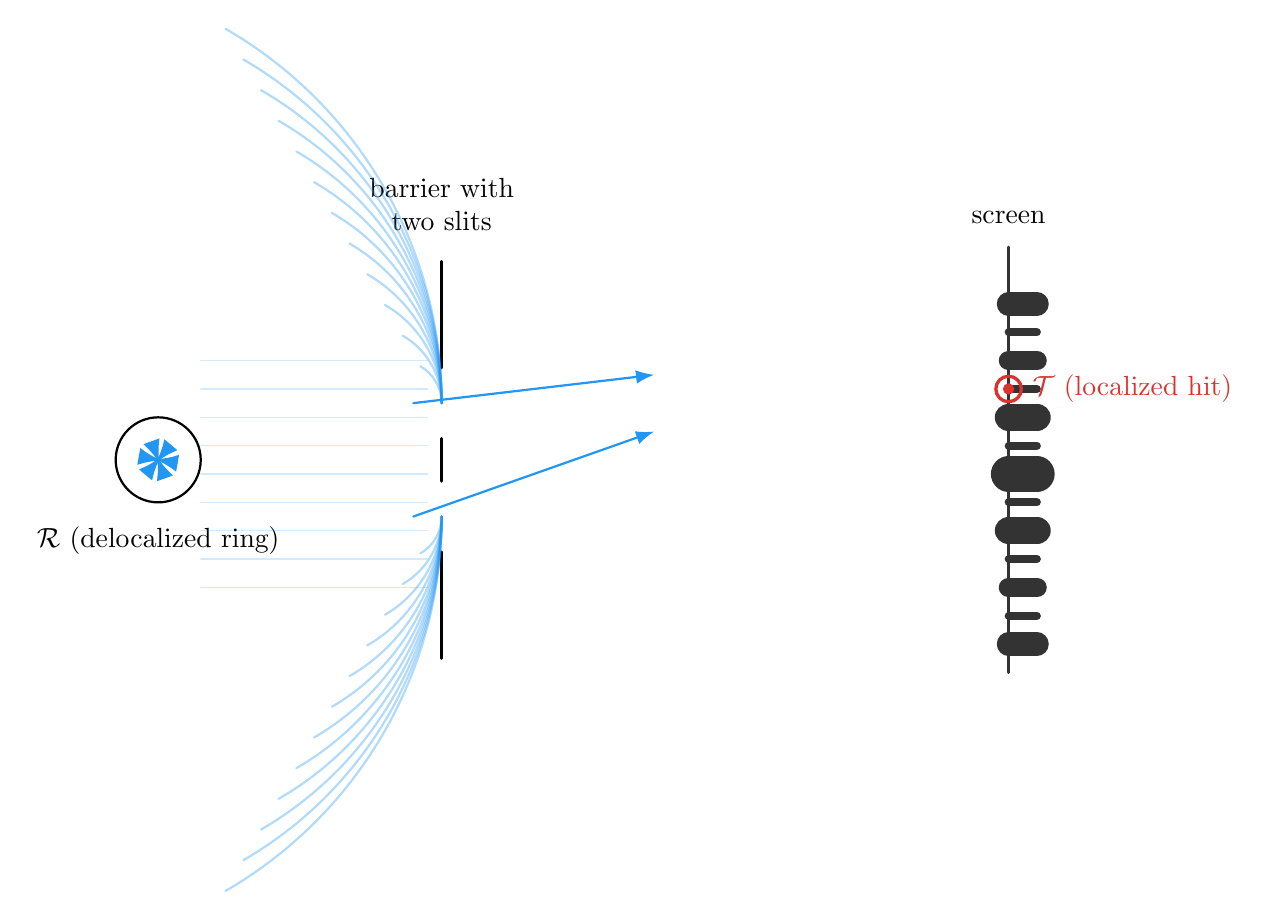
\begin{tikzpicture}[scale=0.9, >=Latex, line cap=round, line join=round]
        % Colors (adjust to grayscale if desired)
    \definecolor{flow}{RGB}{33,150,243}    % coherent flow / phase
    \definecolor{emph}{RGB}{220,50,47}     % localized hit
    \definecolor{screen}{gray}{0.20}

    % --- Source: toroidal circulation (delocalized ring R) ---
    \draw[thick] (-1,0) circle (0.6);
    % circulation arrows along the ring
    \foreach \a in {20,80,140,200,260,320}{
        \draw[->,flow,very thick]
        (-1,0) + ({0.6*cos(\a)},{0.6*sin(\a)})
        ++({-0.20*sin(\a)},{0.20*cos(\a)}) -- ++({0.25*sin(\a)},{-0.25*cos(\a)});
    }
    \node[below] at (-1,-0.8) {$\mathcal R$ (delocalized ring)};

    % --- Barrier with two slits ---
    \draw[very thick] (3,-2.8) -- (3,-1.3);
    \draw[very thick] (3,-0.3) -- (3,0.3);
    \draw[very thick] (3,1.3) -- (3,2.8);
    \node[above, align=center] at (3,3.1) {barrier with\\two slits};

    % --- Screen ---
    \draw[very thick,screen] (11,-3) -- (11,3);
    \node[above] at (11,3.2) {screen};

    % --- Incident phase field toward slits (schematic parallel rays) ---
    \foreach \y in {-1.8,-1.4,...,1.8}{
        \draw[flow,opacity=0.20] (-0.4,\y) -- (2.8,\y);
    }

    % --- Huygens-like secondary wavelets from each slit (schematic arcs) ---
    \foreach \r in {0.6,1.1,1.6,2.1,2.6,3.1,3.6,4.1,4.6,5.1,5.6,6.1}{
        \draw[flow,thick,opacity=0.35] (3, 0.8) arc (0:60:\r);
        \draw[flow,thick,opacity=0.35] (3,-0.8) arc (0:-60:\r);
    }

    % --- Interference intensity on the screen: alternating thicker ticks ---
    \foreach \yy/\wid in {-2.6/0.30,-2.2/0.10,-1.8/0.25,-1.4/0.10,-1.0/0.35,
    -0.6/0.10,-0.2/0.45, 0.2/0.10, 0.6/0.35, 1.0/0.10,
    1.4/0.25, 1.8/0.10, 2.2/0.30}{
        \draw[screen,line width=\wid cm] (11,\yy) -- ++(0.40,0);
    }

    % --- Localized detection (collapse to T) ---
    \fill[emph] (11,1.0) circle (0.08);
    \draw[emph,very thick] (11,1.0) circle (0.18);
    \node[right,emph] at (11.2,1.0) {$\mathcal T$ (localized hit)};

    % --- Two representative coherent paths (guiding arrows) ---
    \draw[->,flow,thick] (2.6, 0.8) -- (6,1.2);
    \draw[->,flow,thick] (2.6,-0.8) -- (6,0.4);
    \end{tikzpicture}
    \caption{SST double slit schematic. The electron approaches as a delocalized toroidal circulation $\mathcal R$ (ring), whose phase bifurcates at two slits to produce coherent downstream fields that interfere. At the screen, interaction triggers collapse into a localized knotted state $\mathcal T$, yielding discrete impacts while the ensemble reproduces the fringe intensity.}
    \label{fig:SST-double-slit}
    \end{figure}

%===============================
% Extended Analysis Sections
%===============================

\section{Quantitative Fringe Geometry and Visibility}

    Consider a double slit with center-to-center separation $s$ and distance $L$ from slits to screen.
    Let the electron approach in the delocalized ring phase $\mathcal R$ with mean axial momentum $p_z$ (de Broglie wavelength $\lambda=h/p_z$).
    In the Fraunhofer regime ($L \gg s^2/\lambda$), the transverse intensity on the screen is well approximated by
    \begin{equation}
    I(x) \;\propto\; I_1(x) + I_2(x) + 2\sqrt{I_1(x)I_2(x)}\,\cos\!\Big(\tfrac{2\pi s}{\lambda}\tfrac{x}{L} + \phi_0\Big),
    \end{equation}
    with fringe spacing
    \begin{equation}
    \boxed{\ d \;=\; \frac{\lambda L}{s}\ }.
    \end{equation}
    Within SST, the phase $\phi_0$ is the circulation phase offset inherited from $\mathcal R$; any path-dependent coupling to the environment adds a random phase $\delta\phi$ that reduces the fringe visibility
    \begin{equation}
    \mathcal V \equiv \frac{I_{\max}-I_{\min}}{I_{\max}+I_{\min}} \;=\; \big|\langle e^{i \delta\phi}\rangle\big|.
    \end{equation}

    \subsection{Ring-phase mapping}
        For the ring state $\mathcal R$ with quantized azimuthal phase $e^{i n\theta}$, the two slits act as partial projectors of this phase onto two spatially separated downstream wavefronts. The resulting interference encodes the \emph{same} azimuthal winding through the optical path difference $\Delta \ell(x) \approx s\,x/L$, hence the cosine argument above.

\section{Which-Way Coupling and Decoherence in SST}

    In SST language, ``which-way'' monitoring is an \emph{EM impedance} to the ring phase, parameterized by a coupling rate $\Gamma$ (net photon or field-interaction rate that carries path information).
    Let $\tau$ be the transit time through the interferometer.
    For weak, memoryless monitoring the phase undergoes a random walk, giving the standard exponential visibility law~\cite{Zurek2003}
    \begin{equation}
    \boxed{\ \mathcal V(\Gamma,\tau) \;=\; e^{-\Gamma \tau}\ }. \label{eq:Vexp}
    \end{equation}
    Equivalently, define a \emph{monitoring strength} $\eta\in[0,1]$ as the single-pass which-way information; then $\mathcal V=\sqrt{1-\eta}$ (two-outcome, information-balance form). Both parameterizations are compatible at small $\eta$ via $\eta\simeq 2(1-e^{-\Gamma\tau})$.

    \paragraph{SST mechanism.}
        Microscopically, the EM coupling stochastically seeds premature $\mathcal R\!\to\!\mathcal T$ collapses \emph{upstream}, terminating coherent superposition.
        Equation~\eqref{eq:Vexp} thus measures the survival probability of coherence before the knotting transition.

\subsection{Dimensional check}
$\Gamma$ has units s$^{-1}$ and $\tau$ has units s, so $\Gamma\tau$ is dimensionless, consistent with~\eqref{eq:Vexp}.

\section{Delayed-Choice and Quantum Eraser (SST View)}

In a Wheeler-type delayed choice, the interferometer is reconfigured \emph{after} the electron passes the slits~\cite{Wheeler1978}.
In SST, this reconfiguration alters whether the downstream optics \emph{allow} continued $\mathcal R$-phase recombination or instead force local $\mathcal T$-phase collapse:
\begin{itemize}
\item \textbf{Interference mode on:} downstream optics preserve the $\mathcal R$ phase coherence until the screen $\Rightarrow$ fringes.
\item \textbf{Which-way mode on:} downstream optics couple EM impedance strongly, enforcing premature $\mathcal R\!\to\!\mathcal T$ collapse $\Rightarrow$ no fringes.
\end{itemize}
A quantum eraser removes the stored which-way information, effectively \emph{post-selecting} runs where $\mathcal R$-coherence survived to the recombination stage; sorted sub-ensembles then display fringes.

\section{Spectroscopic Rabi Drive Between $\mathcal R$ and $\mathcal T$}

We model the $\mathcal R\leftrightarrow\mathcal T$ manifold as a driven two-level system with detuning $\Delta=\omega-\omega_0$ (where $\hbar\omega_0=\Delta E_{\mathcal R\to\mathcal T}$) and coupling $\Omega_R$ set by the EM impedance overlap:
\begin{align}
\dot c_{\mathcal R} &= -\tfrac{i}{2}\Omega_R c_{\mathcal T} - \tfrac{\gamma_{\mathcal R}}{2} c_{\mathcal R},\\
\dot c_{\mathcal T} &= -\tfrac{i}{2}\Omega_R c_{\mathcal R} - \Big(\tfrac{\gamma_{\mathcal T}}{2} + i\Delta\Big) c_{\mathcal T}.
\end{align}
At resonance ($\Delta=0$) and for $\gamma_{\mathcal R},\gamma_{\mathcal T}\ll \Omega_R$,
\begin{equation}
P_{\mathcal T}(t)=|c_{\mathcal T}(t)|^2 \;=\; \sin^2\!\Big(\frac{\Omega_R t}{2}\Big)\,e^{-\gamma t},\qquad \gamma\equiv\tfrac{\gamma_{\mathcal R}+\gamma_{\mathcal T}}{2}.
\end{equation}
A \emph{pump--probe} synchronized to the flight time across the interferometer can therefore \emph{gate} the knotting probability and modulate fringe visibility in a time-resolved fashion.

%===============================
% Figures (TikZ)
%===============================

\begin{figure}[t]
\centering
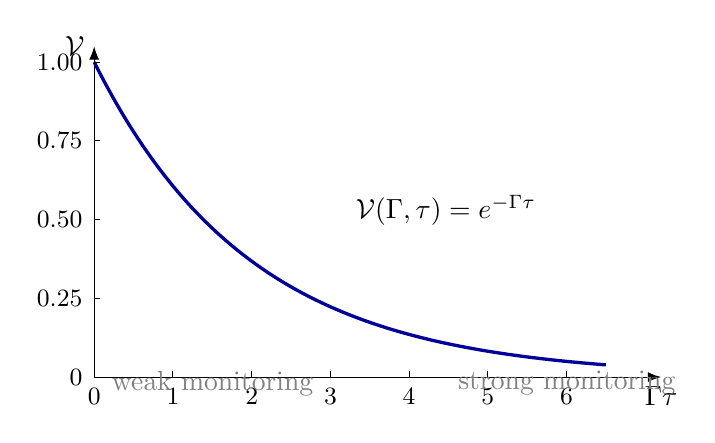
\begin{tikzpicture}[>=Latex,scale=1.0]
    % Axes
\draw[->] (0,0) -- (7.2,0) node[below] {$\Gamma\tau$};
\draw[->] (0,0) -- (0,4.2) node[left] {$\mathcal V$};
% Curve V = exp(-Gamma tau)
\draw[very thick,blue!60!black,domain=0:6.5,samples=200] plot(\x,{4*exp(-0.5*\x)});
% Ticks and labels
\foreach \x/\lab in {0/0,1/1,2/2,3/3,4/4,5/5,6/6}{
    \draw (\x,0) -- ++(0,0.08) node[below,yshift=-3pt] {\small \lab};
}
\foreach \y/\lab in {0/0,1/0.25,2/0.50,3/0.75,4/1.00}{
    \draw (0,\y) -- ++(0.08,0) node[left,xshift=-3pt] {\small \lab};
}
\node[above right] at (3.2,1.8) {$\mathcal V(\Gamma,\tau)=e^{-\Gamma\tau}$};
\node[below right,gray] at (0.1,0.2) {weak monitoring};
\node[below right,gray] at (4.5,0.2) {strong monitoring};
\end{tikzpicture}
\caption{Fringe visibility vs.\ which-way coupling in SST.
The parameter $\Gamma$ encodes EM impedance to the $\mathcal R$ phase (path information rate),
    $\tau$ is the transit time.
    Exponential decay of visibility reflects coherence loss prior to recombination.}
\label{fig:VvsGamma}
\end{figure}

\begin{figure}[t]
\centering
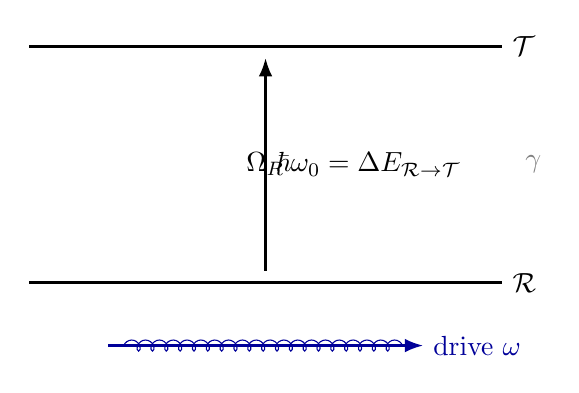
\begin{tikzpicture}[>=Latex,scale=1.0]
    % Energy levels
\draw[very thick] (0,0) -- (6,0) node[right] {$\mathcal R$};
\draw[very thick] (0,3) -- (6,3) node[right] {$\mathcal T$};
% Transition arrow
\draw[->,thick] (3,0.15) -- node[right] {$\hbar\omega_0=\Delta E_{\mathcal R\to\mathcal T}$} (3,2.85);
% Driving field
\draw[->,thick,blue!60!black] (1,-0.8) -- (5,-0.8) node[right] {drive $\omega$};
\draw[blue!60!black,decorate,decoration={coil,aspect=0.8,segment length=5pt,amplitude=2pt}] (1.2,-0.8) -- (4.8,-0.8);
% Rabi label
\node at (3,1.5) {$\Omega_R$};
% Damping
\node[gray] at (6.4,1.5) {$\gamma$};
\end{tikzpicture}
\caption{Two-level SST manifold for $\mathcal R \leftrightarrow \mathcal T$ with Rabi drive.
At resonance $\omega=\omega_0$, the knotting probability oscillates at $\Omega_R$ and decays at rate $\gamma$, enabling pump--probe control of collapse within an interferometer.}
\label{fig:RabiRT}
\end{figure}

%===============================
% Boxed executive statement
%===============================
\begin{center}
\fbox{\parbox{0.92\linewidth}{
    \textbf{Boxed Result (SST double slit).}
    An electron is a single swirl-string with two phases: $\mathcal R$ (delocalized ring) for propagation and $\mathcal T$ (knotted soliton) for detection.
    Interference arises from coherent splitting and recombination of $\mathcal R$; localized impacts result from $\mathcal R\!\to\!\mathcal T$ collapse at the screen.
    Which-way monitoring increases the EM impedance, raising the premature knotting rate $\Gamma$; the fringe visibility obeys $\mathcal V=e^{-\Gamma\tau}$ and vanishes in the strong-monitoring limit.}}
\end{center}
\bibliographystyle{unsrt}
\begin{thebibliography}{99}

\bibitem{Madelung1927}
E.~Madelung.
\newblock Quantentheorie in hydrodynamischer Form.
\newblock {\em Zeitschrift f{\"u}r Physik}, 40:322--326, 1927.
\newblock doi:10.1007/BF01400372.

\bibitem{deBroglie1925}
L.~de Broglie.
\newblock Recherches sur la th{\'e}orie des quanta.
\newblock {\em Annales de Physique}, 3(10):22--128, 1925.
\newblock doi:10.1051/anphys/192510030022.

\bibitem{Bohm1952a}
D.~Bohm.
\newblock A Suggested Interpretation of the Quantum Theory in Terms of ``Hidden'' Variables I.
\newblock {\em Phys. Rev.}, 85(2):166--179, 1952.
\newblock doi:10.1103/PhysRev.85.166.

\bibitem{Bohm1952b}
D.~Bohm.
\newblock A Suggested Interpretation of the Quantum Theory in Terms of ``Hidden'' Variables II.
\newblock {\em Phys. Rev.}, 85(2):180--193, 1952.
\newblock doi:10.1103/PhysRev.85.180.

\bibitem{Onsager1949}
L.~Onsager.
\newblock Statistical hydrodynamics.
\newblock {\em Il Nuovo Cimento (Supplemento)}, 6:279--287, 1949.
\newblock doi:10.1007/BF02780991.

\bibitem{Feynman1955}
R.~P. Feynman.
\newblock Application of Quantum Mechanics to Liquid Helium.
\newblock In C.~J. Gorter, editor, {\em Progress in Low Temperature Physics, Vol. I}, pages 17--53. North-Holland, 1955.
\newblock doi:10.1016/S0079-6417(08)60077-3.

\bibitem{Helmholtz1858}
H.~von Helmholtz.
\newblock {\"U}ber Integrale der hydrodynamischen Gleichungen, welche den Wirbelbewegungen entsprechen.
\newblock {\em Journal f{\"u}r die reine und angewandte Mathematik}, 55:25--55, 1858.
\newblock doi:10.1515/crll.1858.55.25.

\bibitem{Kelvin1869}
W.~Thomson (Lord Kelvin).
\newblock On Vortex Motion.
\newblock {\em Transactions of the Royal Society of Edinburgh}, 25:217--260, 1869.

\end{thebibliography}

\end{document}